\documentclass{article}
\usepackage{amsmath}
\usepackage{amssymb}
\usepackage{algorithm}
\usepackage{float}
\usepackage{color}
\usepackage{multicol}
\usepackage{forloop}
\usepackage{graphicx}
\usepackage[margin=0.8in]{geometry}
\usepackage{caption}
\usepackage{enumerate}

\graphicspath{ {.} }
\title{COMP 4106\\
	\large{Final Project, Blackjack AI (GA and MCTS)}}
\author{Krystian Wojcicki, 101001444}
\date{Winter 2020}

\begin{document}
\maketitle

\section{Description}
Blackjack, also known as Twenty One, is a card game played between one or more players and a dealer where each player in turn competes against the dealer. Players do not compete against each other and aside from using cards from the same deck, do not impact themselves. 

\begin{figure}[H]
\centerline{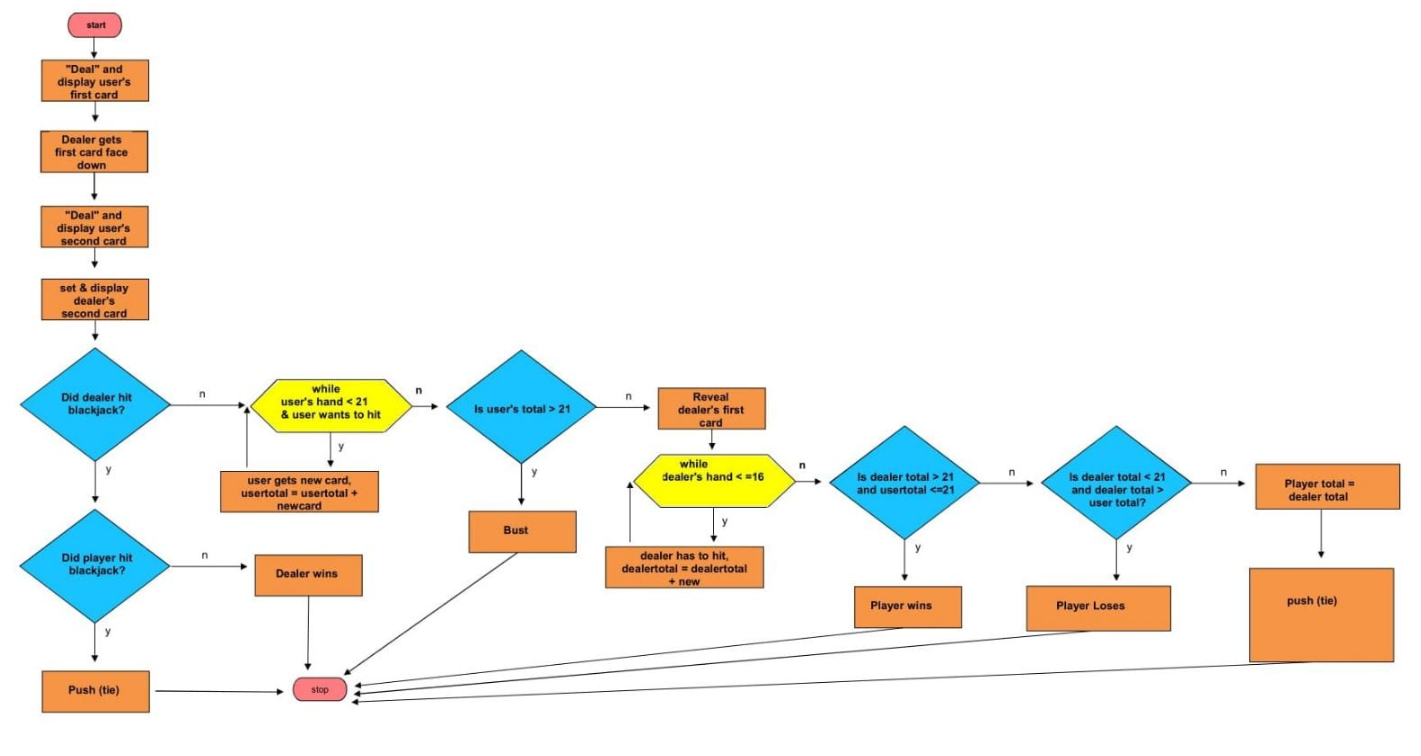
\includegraphics[scale=0.55]{flowchart}}
\caption{Flowchart for Blackjack}
\label{fig:blackjack}
\end{figure}

As can be seen from figure \ref{fig:blackjack} the rules of the game are not too complex, but still complex enough to not have an obvious strategy. The rules for the dealer are given as a fact so the game can be simulated. 

\section{Motivation}
In class several techniques were taught in how to deal with one and two player games: minimax, A*, bfs etc. The problem with these methods was all moves had an equal chance of occurring. In the game of Blackjack depending on the dealers cards and your cards, the probability of of receiving a specific card when "hitting" differs. In addition unlike say in chess or Mancala, there is hidden information. One cannot see the other dealers card. I thought learning how to deal with these uncertainties would be an interesting and challenging problem. 

\section{AI Techniques}
Two techniques will be investigated Genetic Algorithms, GA, and Monte-Carlo Tree Search, MCTS \cite{ga}\cite{mcts}. 

At a high level GA's is a search heuristic that utilizes a survival of the fitness technique for obtaining a solution. An initial population is created randomly, where in this case each individual has a slightly different strategy for playing various Blackjack hands, the individuals with the highest fitness (measured by return on value) are breed. This cycle of selection, mutation and crossover is continued until a stop criteria, either a maximum number of iterations or the fitness reaches some maximum. This technique is often utilized for optimization problems where an optimal solution is not necessary and a near optimal solution is acceptable. 

MCTS have some similarity to the MiniMax algorithm taught in class. In MiniMax all possible moves were generated an evaluated, excluding those ones pruned by alpha/beta. The primary difference being the production system is replaced by a simulation system. Where the simulation system simulates the game and provides simulated outputs. This allows the search to approximate the chance of a certain event happening, without necessarily actually knowing the probability. 

\begin{figure}[H]
\centerline{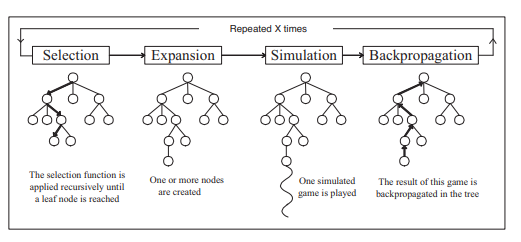
\includegraphics[scale=0.75]{mcts}}
\caption{Outline of a Monte-Carlo Tree Search}
\label{fig:vowpal_wabbit_hash}
\end{figure}


\section{Bibliography}
\begin{thebibliography}{9}

\bibitem{ga} 
Adaptation in Natural and Artificial Systems: An Introductory Analysis with Applications to Biology, Control and Artificial Intelligence, 1992,
Holland, John H

\bibitem{mcts}
Monte-Carlo Tree Search: A New Framework for Game AI, 2008,
Guillaume Chaslot, Sander Bakkes, Istvan Szita and Pieter Spronck
\\\texttt{https://www.aaai.org/Papers/AIIDE/2008/AIIDE08-036.pdf}
\end{thebibliography}

\end{document}